\chapter{Конструкторский раздел}
\label{cha:design}

%\section{Общая архитектура приложения}
%В состав программного обеспечения входит только загружаемый модуль ядра, следящий за вызовом нужных функций, с последующией отправкой информации о них клиенту напрямую из пространства ядра.


%\section{Алгоритмы}

На рисунке \ref{idef0lvl0} показаны входные и выходные потоки данных,
фреймворк и библиотека, необходимые для реализации поставленной задачи.
IDEF0-диаграмма нулевого уровня:

\begin{figure}[h!]
	\centering
	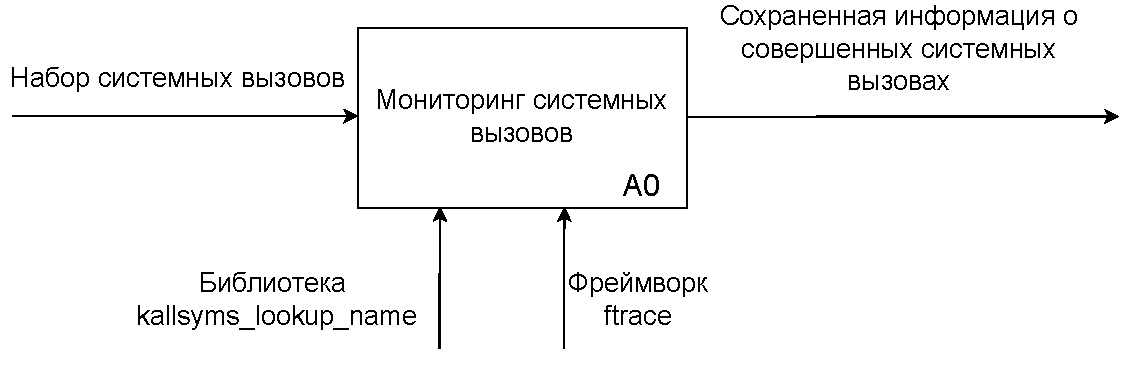
\includegraphics[width=1.0\textwidth]{inc/IDEF0-lvl0.drawio.pdf}
	\caption{IDEF0-диаграмма нулевого уровня}
	\label{idef0lvl0}
\end{figure}

%IDEF0-диаграмма первого уровня (Последовательность действий при мониторинге системных вызовов)

Загружаемый модуль ядра должен обеспечить выполнение следующей
последовательности действий, изображенный на рисунке \ref{idef0lvl1}:

\begin{figure}[h!]
	\centering
	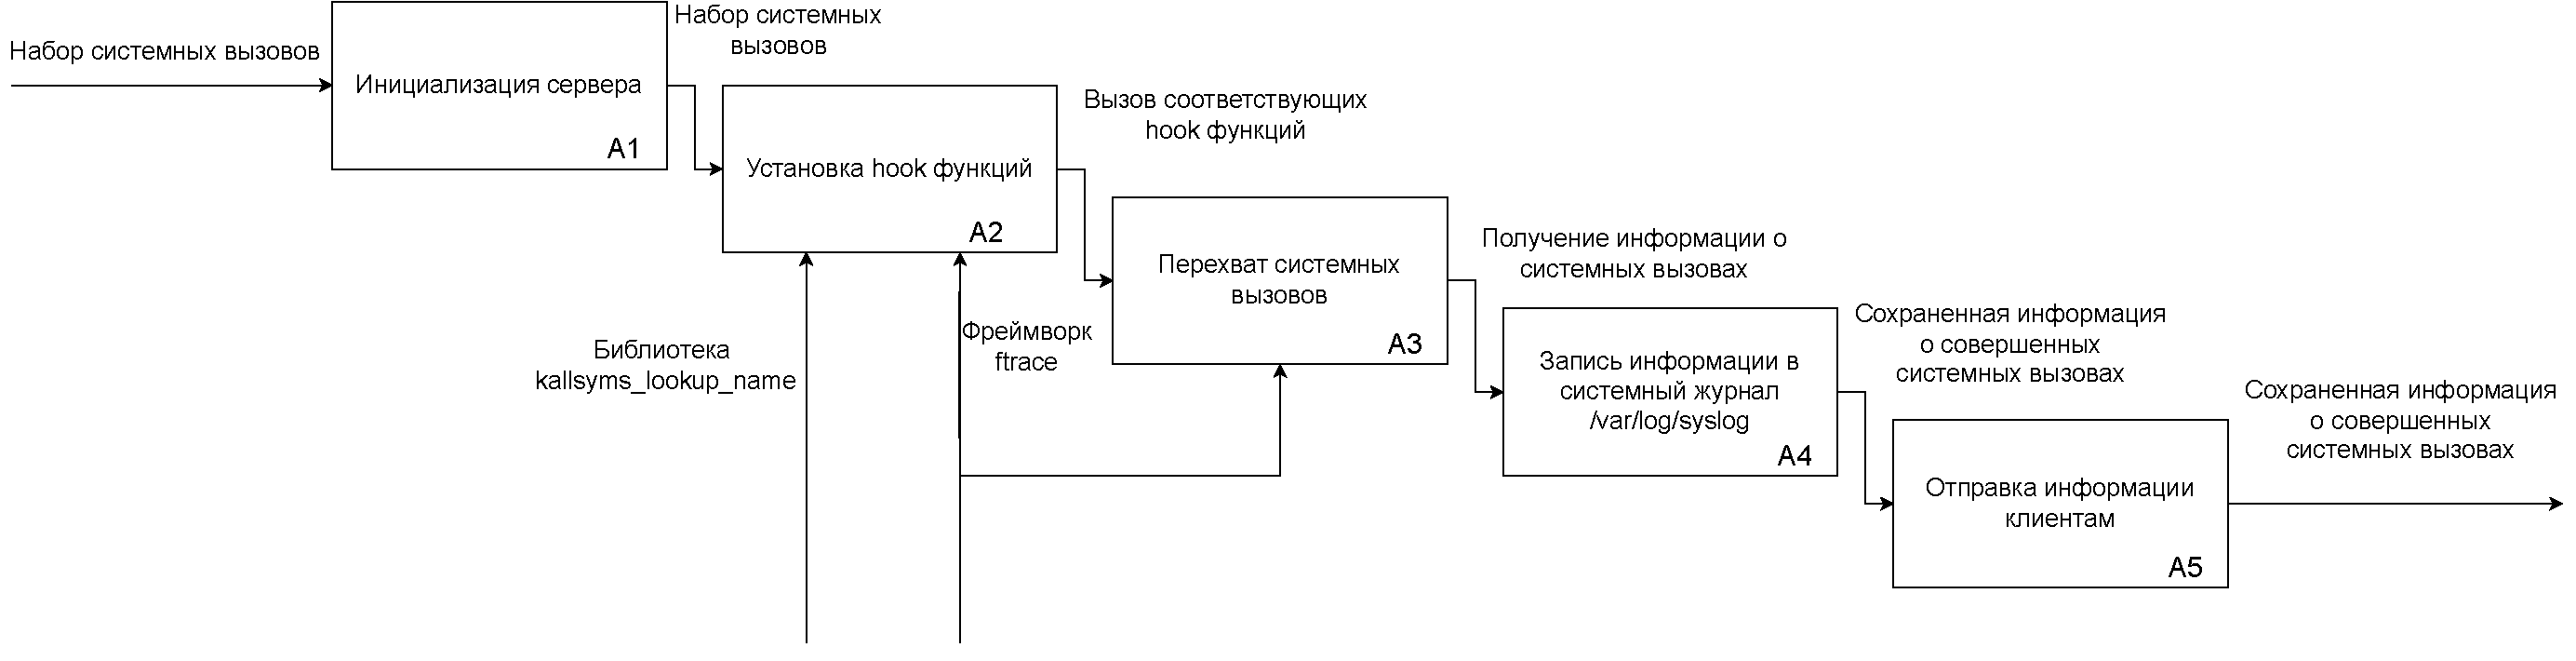
\includegraphics[width=1.0\textwidth]{inc/IDEF0-lvl1.drawio.pdf}
	\caption{IDEF0-диаграмма первого уровня}
	\label{idef0lvl1}
\end{figure}

На первом этапе необходимо установить hook функцию. Далее поток системных вызовов перехватывается нашими hook функциями, и информация записывается в системный журнал /var/log/syslog.

\newpage
\section{Схемы алгоритмов}

%Схемы + немного текста

%\subsection{Алгоритм перехвата функции}
На рисунке \ref{alg1} представлен алгоритм работы перехвата системного
вызовы при использовании ftrace.

\begin{figure}[h!]
	\centering
	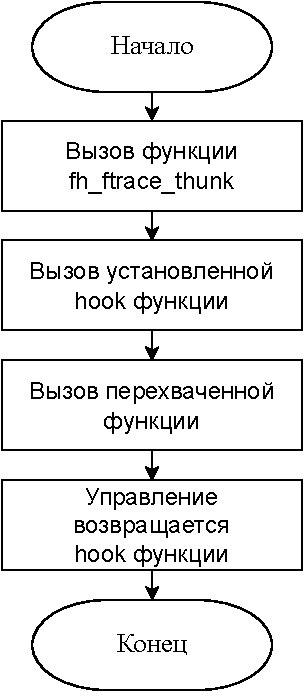
\includegraphics[width=0.3\textwidth]{inc/alg1.drawio.pdf}
	\caption{Алгоритм перехвата функций}
	\label{alg1}
\end{figure}

Пользовательский процесс вызывает макрос SYSCALL. Макрос
переводит систему в режим ядра и управление передаётся низкоуровневому
обработчику системных вызовов — entry\_SYSCALL\_64(). Управление
переходит к конкретному обработчику. Ядро передаёт управление
высокоуровневой функции do\_syscall\_64(). Эта функция в свою очередь
обращается к таблице обработчиков системных вызовов sys\_call\_table и
вызывает конкретный обработчик по номеру системного вызова. В
начале каждой функции ядра находится вызов функции \_\_fentry\_\_(), которая
выполняет защиту от зацикливания и реализуется фреймворком ftrace.
Ftrace вызывает установленную callback-функцию, которая выполняет
перехват. Далее управление с помощью безусловного перехода передаётся
установленной обёрточной функции. При этом состояние процессора и памяти
остаётся неизменным, поэтому данная функция получает все аргументы
исходного системного вызова и при завершении вернёт управление в функцию
do\_syscall\_64(). Обёрточная функция может проанализировать аргументы и
контекст системного вызова и запретить или разрешить процессу его
выполнение. В случае запрета функция просто возвращает код ошибки. Иначе
происходит вызов исходной функции ядра, которая вызывается повторно,
через указатель, который был сохранён при настройке перехвата, после чего
системный вызов завершается и управление передаётся пользовательскому
процессу.

%\subsection{Алгоритм защиты от зацикливания}
В результате работы обёрточной функции происходит повторный вызов
функции ядра, который ftrace также обработает. Для того, чтобы избежать
зацикливания при перехвате функции ядра необходимо проверять, был ли
произведён вызов из текущего модуля, что выполняется функцией
\_\_fentry\_\_(). В случае, когда адрес вызываемой стороны находится в пределах
модуля обёрточная функция не будет вызвана и потому системный вызов
отработает без перехвата. Алгоритм защиты от рекурсивных вызовов показан
на рисунке \ref{alg2}

\begin{figure}[h]
	\centering
	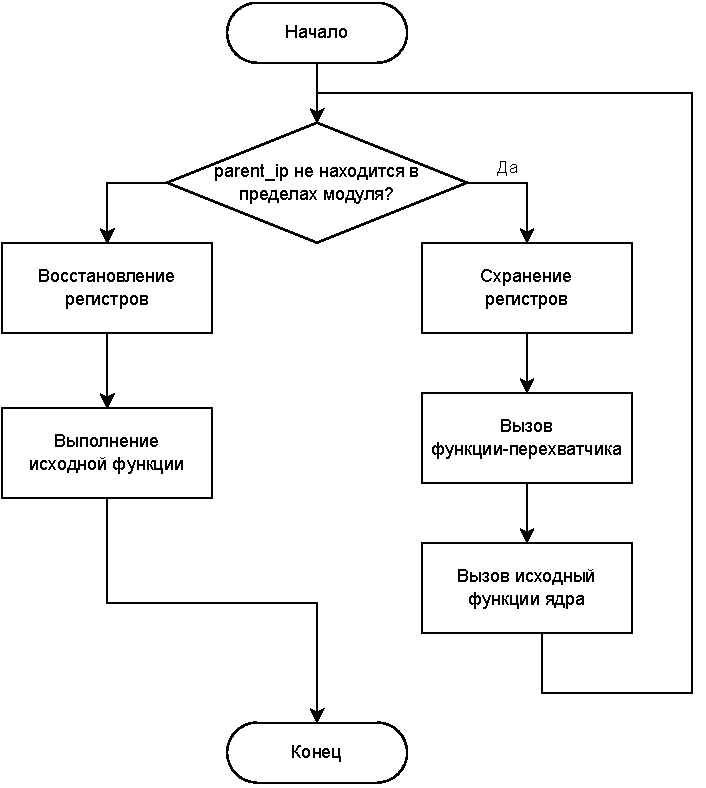
\includegraphics[width=0.7\textwidth]{inc/alg3.drawio.pdf}
	\caption{Алгоритм защиты от зацикливания}
	\label{alg2}
\end{figure}

%\newpage
%\section{Алгоритм работы сервера}
%При загрузке модуля, выделяется память под структуры tcp\_server\_service и tcp\_conn\_handler, running устанавливается в 1 и создается поток, слушающий, все приходящие соединения. Этому потоку передается на вход функция tcp\_server\_listen, которая делает стандартную последовательность действий для любого сервера, а именно: заполняет структуру sockaddr\_in, далее вызывает функции bind и listen. После создается новый поток для принятия соединений, ему на вход передается функция tcp\_server\_accept. Ранее созданный поток переходит в режим ожидания событий. 
%
%Соединения на сервере работают по принципу keep-alive, это значит, что не рвется соединение с клиентом, а постоянно что-то записывается в сокет. Поэтому необходимо, чтобы клиенты не блокировали друг-друга. После того, как соединение принято функцией accept и заполнился сокет для каждого клиента, обработка соединения передается новому потоку, чтобы можно было принимать клиентов дальше.
%
%Преимущества подхода:
%\begin{itemize}
%	\item Клиенты не блокируют и не ждут друг-друга
%	\item Клиенты никак не взаимодействуют между собой
%	\item Падение клиента не влияет на работу системы
%\end{itemize}
%
%Недостатки:
%\begin{itemize}
%	\item На каждого клиента создается новый поток, а значит будет создано N потоков в пространстве ядра на N клиентов. Это несомненно плохо, потому что больше задач будет бороться за получение кванта процессорного времени.
%	\item Отправка данных клиенту происходит из функции перехватчика, поэтому требовуется каким-то образом передать ей данные о соединении. Самый простой способ - глобальный массив клиентов. В этом подходе есть существенная проблема: если описать несколько функций перехватчиков и передавать данные одним и тем же клиентам, то будет конкурентный доступ к этому массиву. В функциях перехватчиках нельзя вызывать блокировки, в связи с тем, что они могут повесить систему.
%\end{itemize}
%
%\section{Структура ПО}
%В состав программного обеспечения входит загружаемый модуль ядра, следящий за вызовом нужных функций, с последующией отправкой информации о них клиенту напрямую из пространства ядра.
% Добавить/изменить?

\newpage 
\section{Алгоритм запуска сервера}
При загрузке модуля, выделяется память под структуры tcp\_server\_service и tcp\_conn\_handler и создается поток, слушающий, все приходящие соединения (листинг \ref{network_server_init}). 

\begin{figure}[h]
	\centering
	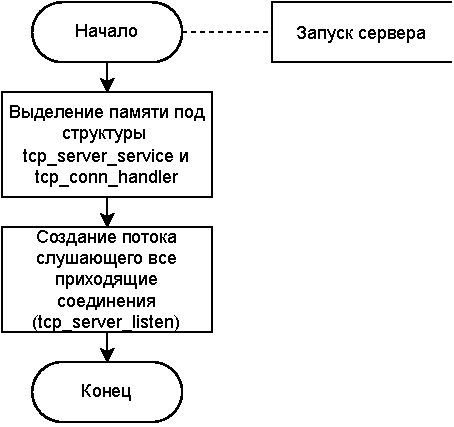
\includegraphics[width=0.4\textwidth]{inc/network_server_init.drawio.pdf}
	\caption{Алгоритм запуска сервера}
	\label{network_server_init}
\end{figure}

Этому потоку передается на вход функция tcp\_server\_listen, которая делает стандартную последовательность действий для любого сервера, а именно: заполняет структуру sockaddr\_in, далее вызывает функции bind и listen. После создается новый поток для принятия соединений, ему на вход передается функция tcp\_server\_accept. Ранее созданный поток переходит в режим ожидания событий (листинг \ref{tcp_server_listen}). 

\begin{figure}[h]
	\centering
	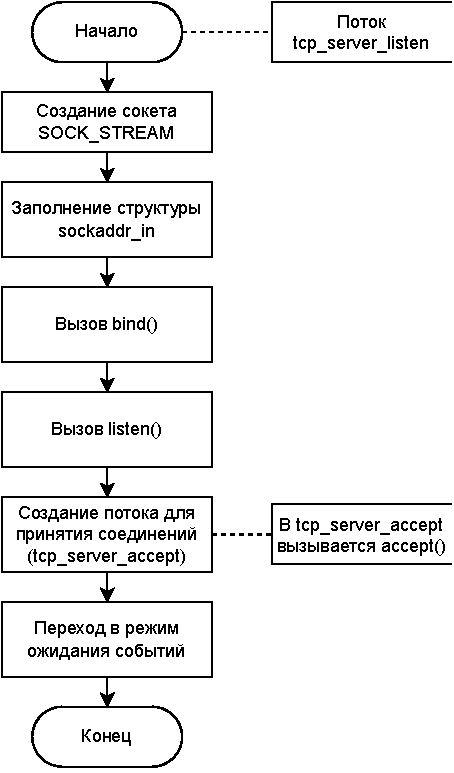
\includegraphics[width=0.3\textwidth]{inc/tcp_server_listen.drawio.pdf}
	\caption{Алгоритм потока слушающего все приходящие соединения}
	\label{tcp_server_listen}
\end{figure}

Соединения на сервере работают по принципу keep-alive, это значит, что не рвется соединение с клиентом, а постоянно что-то записывается в сокет. Поэтому необходимо, чтобы клиенты не блокировали друг-друга. После того, как соединение принято функцией accept, обработка соединения передается новому потоку, чтобы можно было принимать клиентов дальше.

Преимущества подхода:
\begin{itemize}
	\item Клиенты не блокируют и не ждут друг-друга
	\item Клиенты никак не взаимодействуют между собой
	\item Падение клиента не влияет на работу системы
\end{itemize}

Но на каждого клиента создается новый поток, а значит будет создано N потоков в пространстве ядра на N клиентов. Это несомненно является недостатком, потому что больше задач будет бороться за получение кванта процессорного времени.

%Недостатки:
%\begin{itemize}
%	\item На каждого клиента создается новый поток, а значит будет создано N потоков в пространстве ядра на N клиентов. Это несомненно плохо, потому что больше задач будет бороться за получение кванта процессорного времени.
%	\item Отправка данных клиенту происходит из функции перехватчика, поэтому требуется каким-то образом передать ей данные о соединении. Самый простой способ - глобальный массив клиентов. В этом подходе есть существенная проблема: если описать несколько функций перехватчиков и передавать данные одним и тем же клиентам, то будет конкурентный доступ к этому массиву. В функциях перехватчиках нельзя вызывать блокировки, в связи с тем, что они могут повесить систему.
%\end{itemize}

\section{Структура программного обеспечения}
При срабатывании системного вызова из списка отслеживаемых, информация о нем записыфвается в системный журнал и отправляется подключенным клиентам с помощью сервера (рисунок \ref{structurePO}). Таким образом, можно следить за вызовами функций ядра Linux удаленно.

\begin{figure}[h]
	\centering
	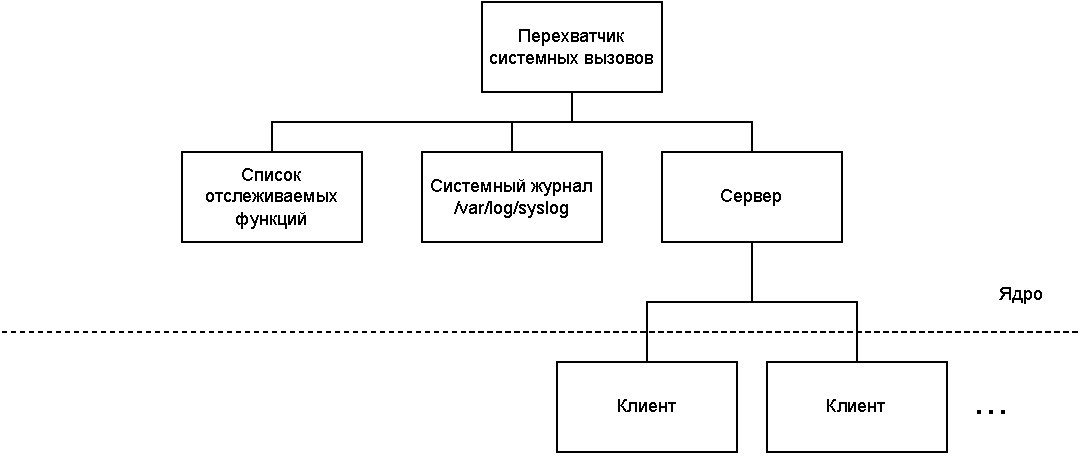
\includegraphics[width=1\textwidth]{inc/structurePO.pdf}
	\caption{Структура ПО}
	\label{structurePO}
\end{figure}

%%% Local Variables:

%%% mode: latex
%%% TeX-master: "rpz"
%%% End:
%--количество цветов
%||количество пикселей